% Copyright © 2013 Martin Ueding <dev@martin-ueding.de>
%
% Copyright © 2012-2013 Martin Ueding <dev@martin-ueding.de>

% This is my general purpose LaTeX header file for writing German documents.
% Ideally, you include this using a simple ``% Copyright © 2012-2013 Martin Ueding <dev@martin-ueding.de>

% This is my general purpose LaTeX header file for writing German documents.
% Ideally, you include this using a simple ``% Copyright © 2012-2013 Martin Ueding <dev@martin-ueding.de>

% This is my general purpose LaTeX header file for writing German documents.
% Ideally, you include this using a simple ``\input{header.tex}`` in your main
% document and start with ``\title`` and ``\begin{document}`` afterwards.

% If you need to add additional packages, I recommend not doing this in this
% file, but in your main document. That way, you can just drop in a new
% ``header.tex`` and get all the new commands without having to merge manually.

% Since this file encorporates a CC-BY-SA fragment, this whole files is
% licensed under the CC-BY-SA license.

\documentclass[11pt, ngerman, fleqn, DIV=15, headinclude]{scrartcl}

\usepackage{graphicx}

% Environment to quote the problem. Currently, this is just a new name for the
% quote environment.
\newenvironment{problem}{\begin{quote}}{\end{quote}}

%%%%%%%%%%%%%%%%%%%%%%%%%%%%%%%%%%%%%%%%%%%%%%%%%%%%%%%%%%%%%%%%%%%%%%%%%%%%%%%
%                                Locale, date                                 %
%%%%%%%%%%%%%%%%%%%%%%%%%%%%%%%%%%%%%%%%%%%%%%%%%%%%%%%%%%%%%%%%%%%%%%%%%%%%%%%

\usepackage{babel}
\usepackage[iso]{isodate}

%%%%%%%%%%%%%%%%%%%%%%%%%%%%%%%%%%%%%%%%%%%%%%%%%%%%%%%%%%%%%%%%%%%%%%%%%%%%%%%
%                          Margins and other spacing                          %
%%%%%%%%%%%%%%%%%%%%%%%%%%%%%%%%%%%%%%%%%%%%%%%%%%%%%%%%%%%%%%%%%%%%%%%%%%%%%%%

\usepackage[parfill]{parskip}
\usepackage{setspace}
\usepackage[activate]{microtype}

\setlength{\columnsep}{2cm}

%%%%%%%%%%%%%%%%%%%%%%%%%%%%%%%%%%%%%%%%%%%%%%%%%%%%%%%%%%%%%%%%%%%%%%%%%%%%%%%
%                                    Color                                    %
%%%%%%%%%%%%%%%%%%%%%%%%%%%%%%%%%%%%%%%%%%%%%%%%%%%%%%%%%%%%%%%%%%%%%%%%%%%%%%%

\usepackage[usenames, dvipsnames]{xcolor}

\colorlet{darkred}{red!70!black}
\colorlet{darkblue}{blue!70!black}
\colorlet{darkgreen}{green!40!black}

%%%%%%%%%%%%%%%%%%%%%%%%%%%%%%%%%%%%%%%%%%%%%%%%%%%%%%%%%%%%%%%%%%%%%%%%%%%%%%%
%                         Font and font like settings                         %
%%%%%%%%%%%%%%%%%%%%%%%%%%%%%%%%%%%%%%%%%%%%%%%%%%%%%%%%%%%%%%%%%%%%%%%%%%%%%%%

% This replaces all fonts with Bitstream Charter, Bitstream Vera Sans and
% Bitstream Vera Mono. Math will be rendered in Charter.
\usepackage[charter, greekuppercase=italicized]{mathdesign}
\usepackage{beramono}
\usepackage{berasans}

% Bold, sans-serif tensors. This fragment is taken from “egreg” from
% http://tex.stackexchange.com/a/82747/8945 and licensed under `CC-BY-SA
% <https://creativecommons.org/licenses/by-sa/3.0/>`_.
\usepackage{bm}
\DeclareMathAlphabet{\mathsfit}{\encodingdefault}{\sfdefault}{m}{sl}
\SetMathAlphabet{\mathsfit}{bold}{\encodingdefault}{\sfdefault}{bx}{sl}
\newcommand{\tens}[1]{\bm{\mathsfit{#1}}}

% Bold vectors.
\renewcommand{\vec}[1]{\boldsymbol{#1}}

%%%%%%%%%%%%%%%%%%%%%%%%%%%%%%%%%%%%%%%%%%%%%%%%%%%%%%%%%%%%%%%%%%%%%%%%%%%%%%%
%                               Input encoding                                %
%%%%%%%%%%%%%%%%%%%%%%%%%%%%%%%%%%%%%%%%%%%%%%%%%%%%%%%%%%%%%%%%%%%%%%%%%%%%%%%

\usepackage[T1]{fontenc}
\usepackage[utf8]{inputenc}

%%%%%%%%%%%%%%%%%%%%%%%%%%%%%%%%%%%%%%%%%%%%%%%%%%%%%%%%%%%%%%%%%%%%%%%%%%%%%%%
%                         Hyperrefs and PDF metadata                          %
%%%%%%%%%%%%%%%%%%%%%%%%%%%%%%%%%%%%%%%%%%%%%%%%%%%%%%%%%%%%%%%%%%%%%%%%%%%%%%%

\usepackage{hyperref}
\usepackage{lastpage}

% This sets the author in the properties of the PDF as well. If you want to
% change it, just override it with another ``\hypersetup`` call.
\hypersetup{
	breaklinks=false,
	citecolor=darkgreen,
	colorlinks=true,
	linkcolor=darkblue,
	menucolor=black,
	pdfauthor={Martin Ueding},
	urlcolor=darkblue,
}

%%%%%%%%%%%%%%%%%%%%%%%%%%%%%%%%%%%%%%%%%%%%%%%%%%%%%%%%%%%%%%%%%%%%%%%%%%%%%%%
%                               Math Operators                                %
%%%%%%%%%%%%%%%%%%%%%%%%%%%%%%%%%%%%%%%%%%%%%%%%%%%%%%%%%%%%%%%%%%%%%%%%%%%%%%%

% AMS environments like ``align`` and theorems like ``proof``.
\usepackage{amsmath}
\usepackage{amsthm}

% Common math constructs like partial derivatives.
\usepackage{commath}

% Physical units.
\usepackage[output-decimal-marker={,}]{siunitx}

% Word like operators.
\DeclareMathOperator{\acosh}{arcosh}
\DeclareMathOperator{\arcosh}{arcosh}
\DeclareMathOperator{\arcsinh}{arsinh}
\DeclareMathOperator{\arsinh}{arsinh}
\DeclareMathOperator{\asinh}{arsinh}
\DeclareMathOperator{\card}{card}
\DeclareMathOperator{\csch}{cshs}
\DeclareMathOperator{\diam}{diam}
\DeclareMathOperator{\sech}{sech}
\renewcommand{\Im}{\mathop{{}\mathrm{Im}}\nolimits}
\renewcommand{\Re}{\mathop{{}\mathrm{Re}}\nolimits}

% Fourier transform.
\DeclareMathOperator{\fourier}{\ensuremath{\mathcal{F}}}

% Roman versions of “e” and “i” to serve as Euler's number and the imaginary
% constant.
\newcommand{\ee}{\eup}
\newcommand{\eup}{\mathrm e}
\newcommand{\ii}{\iup}
\newcommand{\iup}{\mathrm i}

% Symbols for the various mathematical fields (natural numbers, integers,
% rational numbers, real numbers, complex numbers).
\newcommand{\C}{\ensuremath{\mathbb C}}
\newcommand{\N}{\ensuremath{\mathbb N}}
\newcommand{\Q}{\ensuremath{\mathbb Q}}
\newcommand{\R}{\ensuremath{\mathbb R}}
\newcommand{\Z}{\ensuremath{\mathbb Z}}

% Shape like operators.
\DeclareMathOperator{\dalambert}{\Box}
\DeclareMathOperator{\laplace}{\bigtriangleup}
\newcommand{\curl}{\vnabla \times}
\newcommand{\divergence}[1]{\inner{\vnabla}{#1}}
\newcommand{\vnabla}{\vec \nabla}

\newcommand{\half}{\frac 12}

% Unit vector (German „Einheitsvektor“).
\newcommand{\ev}{\hat{\vec e}}

% Scientific notation for large numbers.
\newcommand{\e}[1]{\cdot 10^{#1}}

% Mathematician's notation for the inner (scalar, dot) product.
\newcommand{\bracket}[1]{\left\langle #1 \right\rangle}
\newcommand{\inner}[2]{\bracket{#1, #2}}

% Placeholders.
\newcommand{\emesswert}{\del{\messwert \pm \messwert}}
\newcommand{\fehlt}{\textcolor{darkred}{Hier fehlen noch Inhalte.}}
\newcommand{\messwert}{\textcolor{blue}{\square}}
\newcommand{\punkte}{\phantom{xxxxx}}
\newcommand{\punktevon}[1]{\begin{flushright}/ #1\end{flushright}}

% Separator for equations on a single line.
\newcommand{\eqnsep}{,\quad}

% Quantum Mechanics
\newcommand{\braket}[2]{\left\langle #1 \left. \vphantom{#1 #2} \right| #2 \right\rangle}
\newcommand{\braopket}[3]{\left\langle #1 \left. \vphantom{#1 #2 #3} \right| #2 \left. \vphantom{#1 #2 #3} \right| #3 \right\rangle}
\newcommand{\bra}[1]{\left\langle #1 \right|}
\newcommand{\ketbra}[2]{\left| #1 \vphantom{#2} \right\rangle \left\langle #2  \vphantom{#1} \right|}
\newcommand{\ket}[1]{\left| #1 \right\rangle}

%%%%%%%%%%%%%%%%%%%%%%%%%%%%%%%%%%%%%%%%%%%%%%%%%%%%%%%%%%%%%%%%%%%%%%%%%%%%%%%
%                                  Headings                                   %
%%%%%%%%%%%%%%%%%%%%%%%%%%%%%%%%%%%%%%%%%%%%%%%%%%%%%%%%%%%%%%%%%%%%%%%%%%%%%%%

% This will set fancy headings to the top of the page. The page number will be
% accompanied by the total number of pages. That way, you will know if any page
% is missing.
%
% If you do not want this for your document, you can just use
% ``\pagestyle{plain}``.

\usepackage{scrpage2}

\pagestyle{scrheadings}
\automark{section}
\cfoot{\footnotesize{Seite \thepage\ / \pageref{LastPage}}}
\chead{}
\ihead{}
\ohead{\rightmark}
\setheadsepline{.4pt}

%%%%%%%%%%%%%%%%%%%%%%%%%%%%%%%%%%%%%%%%%%%%%%%%%%%%%%%%%%%%%%%%%%%%%%%%%%%%%%%
%                            Bibliography (BibTeX)                            %
%%%%%%%%%%%%%%%%%%%%%%%%%%%%%%%%%%%%%%%%%%%%%%%%%%%%%%%%%%%%%%%%%%%%%%%%%%%%%%%

\newcommand{\bibliographyfile}{../../zentrale_BibTeX/Central}
\bibliographystyle{apalike2}

%%%%%%%%%%%%%%%%%%%%%%%%%%%%%%%%%%%%%%%%%%%%%%%%%%%%%%%%%%%%%%%%%%%%%%%%%%%%%%%
%                                Abbreviations                                %
%%%%%%%%%%%%%%%%%%%%%%%%%%%%%%%%%%%%%%%%%%%%%%%%%%%%%%%%%%%%%%%%%%%%%%%%%%%%%%%

\newcommand{\dhabk}{\mbox{d.\,h.}}

%%%%%%%%%%%%%%%%%%%%%%%%%%%%%%%%%%%%%%%%%%%%%%%%%%%%%%%%%%%%%%%%%%%%%%%%%%%%%%%
%                                  Licences                                   %
%%%%%%%%%%%%%%%%%%%%%%%%%%%%%%%%%%%%%%%%%%%%%%%%%%%%%%%%%%%%%%%%%%%%%%%%%%%%%%%

\usepackage{ccicons}

\newcommand{\ccbysadetext}{%
	\begin{small}
		Dieses Werk bzw. Inhalt steht unter einer
		\href{http://creativecommons.org/licenses/by-sa/3.0/deed.de}{%
			Creative Commons Namensnennung - Weitergabe unter gleichen
		Bedingungen 3.0 Unported Lizenz}.
	\end{small}
}

\newcommand{\ccbysadetitle}{%
	Lizenz: \href{http://creativecommons.org/licenses/by-sa/3.0/deed.de}
	{CC-BY-SA 3.0 \ccbysa}
}
`` in your main
% document and start with ``\title`` and ``\begin{document}`` afterwards.

% If you need to add additional packages, I recommend not doing this in this
% file, but in your main document. That way, you can just drop in a new
% ``header.tex`` and get all the new commands without having to merge manually.

% Since this file encorporates a CC-BY-SA fragment, this whole files is
% licensed under the CC-BY-SA license.

\documentclass[11pt, ngerman, fleqn, DIV=15, headinclude]{scrartcl}

\usepackage{graphicx}

% Environment to quote the problem. Currently, this is just a new name for the
% quote environment.
\newenvironment{problem}{\begin{quote}}{\end{quote}}

%%%%%%%%%%%%%%%%%%%%%%%%%%%%%%%%%%%%%%%%%%%%%%%%%%%%%%%%%%%%%%%%%%%%%%%%%%%%%%%
%                                Locale, date                                 %
%%%%%%%%%%%%%%%%%%%%%%%%%%%%%%%%%%%%%%%%%%%%%%%%%%%%%%%%%%%%%%%%%%%%%%%%%%%%%%%

\usepackage{babel}
\usepackage[iso]{isodate}

%%%%%%%%%%%%%%%%%%%%%%%%%%%%%%%%%%%%%%%%%%%%%%%%%%%%%%%%%%%%%%%%%%%%%%%%%%%%%%%
%                          Margins and other spacing                          %
%%%%%%%%%%%%%%%%%%%%%%%%%%%%%%%%%%%%%%%%%%%%%%%%%%%%%%%%%%%%%%%%%%%%%%%%%%%%%%%

\usepackage[parfill]{parskip}
\usepackage{setspace}
\usepackage[activate]{microtype}

\setlength{\columnsep}{2cm}

%%%%%%%%%%%%%%%%%%%%%%%%%%%%%%%%%%%%%%%%%%%%%%%%%%%%%%%%%%%%%%%%%%%%%%%%%%%%%%%
%                                    Color                                    %
%%%%%%%%%%%%%%%%%%%%%%%%%%%%%%%%%%%%%%%%%%%%%%%%%%%%%%%%%%%%%%%%%%%%%%%%%%%%%%%

\usepackage[usenames, dvipsnames]{xcolor}

\colorlet{darkred}{red!70!black}
\colorlet{darkblue}{blue!70!black}
\colorlet{darkgreen}{green!40!black}

%%%%%%%%%%%%%%%%%%%%%%%%%%%%%%%%%%%%%%%%%%%%%%%%%%%%%%%%%%%%%%%%%%%%%%%%%%%%%%%
%                         Font and font like settings                         %
%%%%%%%%%%%%%%%%%%%%%%%%%%%%%%%%%%%%%%%%%%%%%%%%%%%%%%%%%%%%%%%%%%%%%%%%%%%%%%%

% This replaces all fonts with Bitstream Charter, Bitstream Vera Sans and
% Bitstream Vera Mono. Math will be rendered in Charter.
\usepackage[charter, greekuppercase=italicized]{mathdesign}
\usepackage{beramono}
\usepackage{berasans}

% Bold, sans-serif tensors. This fragment is taken from “egreg” from
% http://tex.stackexchange.com/a/82747/8945 and licensed under `CC-BY-SA
% <https://creativecommons.org/licenses/by-sa/3.0/>`_.
\usepackage{bm}
\DeclareMathAlphabet{\mathsfit}{\encodingdefault}{\sfdefault}{m}{sl}
\SetMathAlphabet{\mathsfit}{bold}{\encodingdefault}{\sfdefault}{bx}{sl}
\newcommand{\tens}[1]{\bm{\mathsfit{#1}}}

% Bold vectors.
\renewcommand{\vec}[1]{\boldsymbol{#1}}

%%%%%%%%%%%%%%%%%%%%%%%%%%%%%%%%%%%%%%%%%%%%%%%%%%%%%%%%%%%%%%%%%%%%%%%%%%%%%%%
%                               Input encoding                                %
%%%%%%%%%%%%%%%%%%%%%%%%%%%%%%%%%%%%%%%%%%%%%%%%%%%%%%%%%%%%%%%%%%%%%%%%%%%%%%%

\usepackage[T1]{fontenc}
\usepackage[utf8]{inputenc}

%%%%%%%%%%%%%%%%%%%%%%%%%%%%%%%%%%%%%%%%%%%%%%%%%%%%%%%%%%%%%%%%%%%%%%%%%%%%%%%
%                         Hyperrefs and PDF metadata                          %
%%%%%%%%%%%%%%%%%%%%%%%%%%%%%%%%%%%%%%%%%%%%%%%%%%%%%%%%%%%%%%%%%%%%%%%%%%%%%%%

\usepackage{hyperref}
\usepackage{lastpage}

% This sets the author in the properties of the PDF as well. If you want to
% change it, just override it with another ``\hypersetup`` call.
\hypersetup{
	breaklinks=false,
	citecolor=darkgreen,
	colorlinks=true,
	linkcolor=darkblue,
	menucolor=black,
	pdfauthor={Martin Ueding},
	urlcolor=darkblue,
}

%%%%%%%%%%%%%%%%%%%%%%%%%%%%%%%%%%%%%%%%%%%%%%%%%%%%%%%%%%%%%%%%%%%%%%%%%%%%%%%
%                               Math Operators                                %
%%%%%%%%%%%%%%%%%%%%%%%%%%%%%%%%%%%%%%%%%%%%%%%%%%%%%%%%%%%%%%%%%%%%%%%%%%%%%%%

% AMS environments like ``align`` and theorems like ``proof``.
\usepackage{amsmath}
\usepackage{amsthm}

% Common math constructs like partial derivatives.
\usepackage{commath}

% Physical units.
\usepackage[output-decimal-marker={,}]{siunitx}

% Word like operators.
\DeclareMathOperator{\acosh}{arcosh}
\DeclareMathOperator{\arcosh}{arcosh}
\DeclareMathOperator{\arcsinh}{arsinh}
\DeclareMathOperator{\arsinh}{arsinh}
\DeclareMathOperator{\asinh}{arsinh}
\DeclareMathOperator{\card}{card}
\DeclareMathOperator{\csch}{cshs}
\DeclareMathOperator{\diam}{diam}
\DeclareMathOperator{\sech}{sech}
\renewcommand{\Im}{\mathop{{}\mathrm{Im}}\nolimits}
\renewcommand{\Re}{\mathop{{}\mathrm{Re}}\nolimits}

% Fourier transform.
\DeclareMathOperator{\fourier}{\ensuremath{\mathcal{F}}}

% Roman versions of “e” and “i” to serve as Euler's number and the imaginary
% constant.
\newcommand{\ee}{\eup}
\newcommand{\eup}{\mathrm e}
\newcommand{\ii}{\iup}
\newcommand{\iup}{\mathrm i}

% Symbols for the various mathematical fields (natural numbers, integers,
% rational numbers, real numbers, complex numbers).
\newcommand{\C}{\ensuremath{\mathbb C}}
\newcommand{\N}{\ensuremath{\mathbb N}}
\newcommand{\Q}{\ensuremath{\mathbb Q}}
\newcommand{\R}{\ensuremath{\mathbb R}}
\newcommand{\Z}{\ensuremath{\mathbb Z}}

% Shape like operators.
\DeclareMathOperator{\dalambert}{\Box}
\DeclareMathOperator{\laplace}{\bigtriangleup}
\newcommand{\curl}{\vnabla \times}
\newcommand{\divergence}[1]{\inner{\vnabla}{#1}}
\newcommand{\vnabla}{\vec \nabla}

\newcommand{\half}{\frac 12}

% Unit vector (German „Einheitsvektor“).
\newcommand{\ev}{\hat{\vec e}}

% Scientific notation for large numbers.
\newcommand{\e}[1]{\cdot 10^{#1}}

% Mathematician's notation for the inner (scalar, dot) product.
\newcommand{\bracket}[1]{\left\langle #1 \right\rangle}
\newcommand{\inner}[2]{\bracket{#1, #2}}

% Placeholders.
\newcommand{\emesswert}{\del{\messwert \pm \messwert}}
\newcommand{\fehlt}{\textcolor{darkred}{Hier fehlen noch Inhalte.}}
\newcommand{\messwert}{\textcolor{blue}{\square}}
\newcommand{\punkte}{\phantom{xxxxx}}
\newcommand{\punktevon}[1]{\begin{flushright}/ #1\end{flushright}}

% Separator for equations on a single line.
\newcommand{\eqnsep}{,\quad}

% Quantum Mechanics
\newcommand{\braket}[2]{\left\langle #1 \left. \vphantom{#1 #2} \right| #2 \right\rangle}
\newcommand{\braopket}[3]{\left\langle #1 \left. \vphantom{#1 #2 #3} \right| #2 \left. \vphantom{#1 #2 #3} \right| #3 \right\rangle}
\newcommand{\bra}[1]{\left\langle #1 \right|}
\newcommand{\ketbra}[2]{\left| #1 \vphantom{#2} \right\rangle \left\langle #2  \vphantom{#1} \right|}
\newcommand{\ket}[1]{\left| #1 \right\rangle}

%%%%%%%%%%%%%%%%%%%%%%%%%%%%%%%%%%%%%%%%%%%%%%%%%%%%%%%%%%%%%%%%%%%%%%%%%%%%%%%
%                                  Headings                                   %
%%%%%%%%%%%%%%%%%%%%%%%%%%%%%%%%%%%%%%%%%%%%%%%%%%%%%%%%%%%%%%%%%%%%%%%%%%%%%%%

% This will set fancy headings to the top of the page. The page number will be
% accompanied by the total number of pages. That way, you will know if any page
% is missing.
%
% If you do not want this for your document, you can just use
% ``\pagestyle{plain}``.

\usepackage{scrpage2}

\pagestyle{scrheadings}
\automark{section}
\cfoot{\footnotesize{Seite \thepage\ / \pageref{LastPage}}}
\chead{}
\ihead{}
\ohead{\rightmark}
\setheadsepline{.4pt}

%%%%%%%%%%%%%%%%%%%%%%%%%%%%%%%%%%%%%%%%%%%%%%%%%%%%%%%%%%%%%%%%%%%%%%%%%%%%%%%
%                            Bibliography (BibTeX)                            %
%%%%%%%%%%%%%%%%%%%%%%%%%%%%%%%%%%%%%%%%%%%%%%%%%%%%%%%%%%%%%%%%%%%%%%%%%%%%%%%

\newcommand{\bibliographyfile}{../../zentrale_BibTeX/Central}
\bibliographystyle{apalike2}

%%%%%%%%%%%%%%%%%%%%%%%%%%%%%%%%%%%%%%%%%%%%%%%%%%%%%%%%%%%%%%%%%%%%%%%%%%%%%%%
%                                Abbreviations                                %
%%%%%%%%%%%%%%%%%%%%%%%%%%%%%%%%%%%%%%%%%%%%%%%%%%%%%%%%%%%%%%%%%%%%%%%%%%%%%%%

\newcommand{\dhabk}{\mbox{d.\,h.}}

%%%%%%%%%%%%%%%%%%%%%%%%%%%%%%%%%%%%%%%%%%%%%%%%%%%%%%%%%%%%%%%%%%%%%%%%%%%%%%%
%                                  Licences                                   %
%%%%%%%%%%%%%%%%%%%%%%%%%%%%%%%%%%%%%%%%%%%%%%%%%%%%%%%%%%%%%%%%%%%%%%%%%%%%%%%

\usepackage{ccicons}

\newcommand{\ccbysadetext}{%
	\begin{small}
		Dieses Werk bzw. Inhalt steht unter einer
		\href{http://creativecommons.org/licenses/by-sa/3.0/deed.de}{%
			Creative Commons Namensnennung - Weitergabe unter gleichen
		Bedingungen 3.0 Unported Lizenz}.
	\end{small}
}

\newcommand{\ccbysadetitle}{%
	Lizenz: \href{http://creativecommons.org/licenses/by-sa/3.0/deed.de}
	{CC-BY-SA 3.0 \ccbysa}
}
`` in your main
% document and start with ``\title`` and ``\begin{document}`` afterwards.

% If you need to add additional packages, I recommend not doing this in this
% file, but in your main document. That way, you can just drop in a new
% ``header.tex`` and get all the new commands without having to merge manually.

% Since this file encorporates a CC-BY-SA fragment, this whole files is
% licensed under the CC-BY-SA license.

\documentclass[11pt, ngerman, fleqn, DIV=15, headinclude]{scrartcl}

\usepackage{graphicx}

% Environment to quote the problem. Currently, this is just a new name for the
% quote environment.
\newenvironment{problem}{\begin{quote}}{\end{quote}}

%%%%%%%%%%%%%%%%%%%%%%%%%%%%%%%%%%%%%%%%%%%%%%%%%%%%%%%%%%%%%%%%%%%%%%%%%%%%%%%
%                                Locale, date                                 %
%%%%%%%%%%%%%%%%%%%%%%%%%%%%%%%%%%%%%%%%%%%%%%%%%%%%%%%%%%%%%%%%%%%%%%%%%%%%%%%

\usepackage{babel}
\usepackage[iso]{isodate}

%%%%%%%%%%%%%%%%%%%%%%%%%%%%%%%%%%%%%%%%%%%%%%%%%%%%%%%%%%%%%%%%%%%%%%%%%%%%%%%
%                          Margins and other spacing                          %
%%%%%%%%%%%%%%%%%%%%%%%%%%%%%%%%%%%%%%%%%%%%%%%%%%%%%%%%%%%%%%%%%%%%%%%%%%%%%%%

\usepackage[parfill]{parskip}
\usepackage{setspace}
\usepackage[activate]{microtype}

\setlength{\columnsep}{2cm}

%%%%%%%%%%%%%%%%%%%%%%%%%%%%%%%%%%%%%%%%%%%%%%%%%%%%%%%%%%%%%%%%%%%%%%%%%%%%%%%
%                                    Color                                    %
%%%%%%%%%%%%%%%%%%%%%%%%%%%%%%%%%%%%%%%%%%%%%%%%%%%%%%%%%%%%%%%%%%%%%%%%%%%%%%%

\usepackage[usenames, dvipsnames]{xcolor}

\colorlet{darkred}{red!70!black}
\colorlet{darkblue}{blue!70!black}
\colorlet{darkgreen}{green!40!black}

%%%%%%%%%%%%%%%%%%%%%%%%%%%%%%%%%%%%%%%%%%%%%%%%%%%%%%%%%%%%%%%%%%%%%%%%%%%%%%%
%                         Font and font like settings                         %
%%%%%%%%%%%%%%%%%%%%%%%%%%%%%%%%%%%%%%%%%%%%%%%%%%%%%%%%%%%%%%%%%%%%%%%%%%%%%%%

% This replaces all fonts with Bitstream Charter, Bitstream Vera Sans and
% Bitstream Vera Mono. Math will be rendered in Charter.
\usepackage[charter, greekuppercase=italicized]{mathdesign}
\usepackage{beramono}
\usepackage{berasans}

% Bold, sans-serif tensors. This fragment is taken from “egreg” from
% http://tex.stackexchange.com/a/82747/8945 and licensed under `CC-BY-SA
% <https://creativecommons.org/licenses/by-sa/3.0/>`_.
\usepackage{bm}
\DeclareMathAlphabet{\mathsfit}{\encodingdefault}{\sfdefault}{m}{sl}
\SetMathAlphabet{\mathsfit}{bold}{\encodingdefault}{\sfdefault}{bx}{sl}
\newcommand{\tens}[1]{\bm{\mathsfit{#1}}}

% Bold vectors.
\renewcommand{\vec}[1]{\boldsymbol{#1}}

%%%%%%%%%%%%%%%%%%%%%%%%%%%%%%%%%%%%%%%%%%%%%%%%%%%%%%%%%%%%%%%%%%%%%%%%%%%%%%%
%                               Input encoding                                %
%%%%%%%%%%%%%%%%%%%%%%%%%%%%%%%%%%%%%%%%%%%%%%%%%%%%%%%%%%%%%%%%%%%%%%%%%%%%%%%

\usepackage[T1]{fontenc}
\usepackage[utf8]{inputenc}

%%%%%%%%%%%%%%%%%%%%%%%%%%%%%%%%%%%%%%%%%%%%%%%%%%%%%%%%%%%%%%%%%%%%%%%%%%%%%%%
%                         Hyperrefs and PDF metadata                          %
%%%%%%%%%%%%%%%%%%%%%%%%%%%%%%%%%%%%%%%%%%%%%%%%%%%%%%%%%%%%%%%%%%%%%%%%%%%%%%%

\usepackage{hyperref}
\usepackage{lastpage}

% This sets the author in the properties of the PDF as well. If you want to
% change it, just override it with another ``\hypersetup`` call.
\hypersetup{
	breaklinks=false,
	citecolor=darkgreen,
	colorlinks=true,
	linkcolor=darkblue,
	menucolor=black,
	pdfauthor={Martin Ueding},
	urlcolor=darkblue,
}

%%%%%%%%%%%%%%%%%%%%%%%%%%%%%%%%%%%%%%%%%%%%%%%%%%%%%%%%%%%%%%%%%%%%%%%%%%%%%%%
%                               Math Operators                                %
%%%%%%%%%%%%%%%%%%%%%%%%%%%%%%%%%%%%%%%%%%%%%%%%%%%%%%%%%%%%%%%%%%%%%%%%%%%%%%%

% AMS environments like ``align`` and theorems like ``proof``.
\usepackage{amsmath}
\usepackage{amsthm}

% Common math constructs like partial derivatives.
\usepackage{commath}

% Physical units.
\usepackage[output-decimal-marker={,}]{siunitx}

% Word like operators.
\DeclareMathOperator{\acosh}{arcosh}
\DeclareMathOperator{\arcosh}{arcosh}
\DeclareMathOperator{\arcsinh}{arsinh}
\DeclareMathOperator{\arsinh}{arsinh}
\DeclareMathOperator{\asinh}{arsinh}
\DeclareMathOperator{\card}{card}
\DeclareMathOperator{\csch}{cshs}
\DeclareMathOperator{\diam}{diam}
\DeclareMathOperator{\sech}{sech}
\renewcommand{\Im}{\mathop{{}\mathrm{Im}}\nolimits}
\renewcommand{\Re}{\mathop{{}\mathrm{Re}}\nolimits}

% Fourier transform.
\DeclareMathOperator{\fourier}{\ensuremath{\mathcal{F}}}

% Roman versions of “e” and “i” to serve as Euler's number and the imaginary
% constant.
\newcommand{\ee}{\eup}
\newcommand{\eup}{\mathrm e}
\newcommand{\ii}{\iup}
\newcommand{\iup}{\mathrm i}

% Symbols for the various mathematical fields (natural numbers, integers,
% rational numbers, real numbers, complex numbers).
\newcommand{\C}{\ensuremath{\mathbb C}}
\newcommand{\N}{\ensuremath{\mathbb N}}
\newcommand{\Q}{\ensuremath{\mathbb Q}}
\newcommand{\R}{\ensuremath{\mathbb R}}
\newcommand{\Z}{\ensuremath{\mathbb Z}}

% Shape like operators.
\DeclareMathOperator{\dalambert}{\Box}
\DeclareMathOperator{\laplace}{\bigtriangleup}
\newcommand{\curl}{\vnabla \times}
\newcommand{\divergence}[1]{\inner{\vnabla}{#1}}
\newcommand{\vnabla}{\vec \nabla}

\newcommand{\half}{\frac 12}

% Unit vector (German „Einheitsvektor“).
\newcommand{\ev}{\hat{\vec e}}

% Scientific notation for large numbers.
\newcommand{\e}[1]{\cdot 10^{#1}}

% Mathematician's notation for the inner (scalar, dot) product.
\newcommand{\bracket}[1]{\left\langle #1 \right\rangle}
\newcommand{\inner}[2]{\bracket{#1, #2}}

% Placeholders.
\newcommand{\emesswert}{\del{\messwert \pm \messwert}}
\newcommand{\fehlt}{\textcolor{darkred}{Hier fehlen noch Inhalte.}}
\newcommand{\messwert}{\textcolor{blue}{\square}}
\newcommand{\punkte}{\phantom{xxxxx}}
\newcommand{\punktevon}[1]{\begin{flushright}/ #1\end{flushright}}

% Separator for equations on a single line.
\newcommand{\eqnsep}{,\quad}

% Quantum Mechanics
\newcommand{\braket}[2]{\left\langle #1 \left. \vphantom{#1 #2} \right| #2 \right\rangle}
\newcommand{\braopket}[3]{\left\langle #1 \left. \vphantom{#1 #2 #3} \right| #2 \left. \vphantom{#1 #2 #3} \right| #3 \right\rangle}
\newcommand{\bra}[1]{\left\langle #1 \right|}
\newcommand{\ketbra}[2]{\left| #1 \vphantom{#2} \right\rangle \left\langle #2  \vphantom{#1} \right|}
\newcommand{\ket}[1]{\left| #1 \right\rangle}

%%%%%%%%%%%%%%%%%%%%%%%%%%%%%%%%%%%%%%%%%%%%%%%%%%%%%%%%%%%%%%%%%%%%%%%%%%%%%%%
%                                  Headings                                   %
%%%%%%%%%%%%%%%%%%%%%%%%%%%%%%%%%%%%%%%%%%%%%%%%%%%%%%%%%%%%%%%%%%%%%%%%%%%%%%%

% This will set fancy headings to the top of the page. The page number will be
% accompanied by the total number of pages. That way, you will know if any page
% is missing.
%
% If you do not want this for your document, you can just use
% ``\pagestyle{plain}``.

\usepackage{scrpage2}

\pagestyle{scrheadings}
\automark{section}
\cfoot{\footnotesize{Seite \thepage\ / \pageref{LastPage}}}
\chead{}
\ihead{}
\ohead{\rightmark}
\setheadsepline{.4pt}

%%%%%%%%%%%%%%%%%%%%%%%%%%%%%%%%%%%%%%%%%%%%%%%%%%%%%%%%%%%%%%%%%%%%%%%%%%%%%%%
%                            Bibliography (BibTeX)                            %
%%%%%%%%%%%%%%%%%%%%%%%%%%%%%%%%%%%%%%%%%%%%%%%%%%%%%%%%%%%%%%%%%%%%%%%%%%%%%%%

\newcommand{\bibliographyfile}{../../zentrale_BibTeX/Central}
\bibliographystyle{apalike2}

%%%%%%%%%%%%%%%%%%%%%%%%%%%%%%%%%%%%%%%%%%%%%%%%%%%%%%%%%%%%%%%%%%%%%%%%%%%%%%%
%                                Abbreviations                                %
%%%%%%%%%%%%%%%%%%%%%%%%%%%%%%%%%%%%%%%%%%%%%%%%%%%%%%%%%%%%%%%%%%%%%%%%%%%%%%%

\newcommand{\dhabk}{\mbox{d.\,h.}}

%%%%%%%%%%%%%%%%%%%%%%%%%%%%%%%%%%%%%%%%%%%%%%%%%%%%%%%%%%%%%%%%%%%%%%%%%%%%%%%
%                                  Licences                                   %
%%%%%%%%%%%%%%%%%%%%%%%%%%%%%%%%%%%%%%%%%%%%%%%%%%%%%%%%%%%%%%%%%%%%%%%%%%%%%%%

\usepackage{ccicons}

\newcommand{\ccbysadetext}{%
	\begin{small}
		Dieses Werk bzw. Inhalt steht unter einer
		\href{http://creativecommons.org/licenses/by-sa/3.0/deed.de}{%
			Creative Commons Namensnennung - Weitergabe unter gleichen
		Bedingungen 3.0 Unported Lizenz}.
	\end{small}
}

\newcommand{\ccbysadetitle}{%
	Lizenz: \href{http://creativecommons.org/licenses/by-sa/3.0/deed.de}
	{CC-BY-SA 3.0 \ccbysa}
}


\usepackage{tikz}
\usetikzlibrary{calc}

\newcommand{\themodul}{physik411}
\newcommand{\thegruppe}{Gruppe 2 -- Florian Seidler}
\newcommand{\theuebung}{9}

\ifoot{\footnotesize{Martin Ueding}}
\ihead{\themodul{} -- Übung \theuebung}
\ofoot{\footnotesize{\thegruppe}}

\def\thesubsection{\thesection\alph{subsection}}

\title{\themodul{} -- Übung \theuebung}
\subtitle{\thegruppe}
\author{
	Martin Ueding \footnote{\href{mailto:mu@uni-bonn.de}{mu@uni-bonn.de}}
}

\hypersetup{
	pdftitle={\themodul {} - Übung \theuebung},
}

\begin{document}

\maketitle

\begin{center}
	\ccbysadetitle
\end{center}

\begin{table}[h]
	\centering
	\begin{tabular}{l*5{|c}}
		Aufgabe
		& \ref 1
		& \ref 2
		& \ref 3
		& \ref 4
		& $\sum$   \\
		\hline
		Punkte
		& \punkte / 7
		& \punkte / 18
		& \punkte / 14
		& \punkte / 10
		& \punkte / 49
	\end{tabular}
\end{table}

%%%%%%%%%%%%%%%%%%%%%%%%%%%%%%%%%%%%%%%%%%%%%%%%%%%%%%%%%%%%%%%%%%%%%%%%%%%%%%%
%                             Chemische Bindungen                             %
%%%%%%%%%%%%%%%%%%%%%%%%%%%%%%%%%%%%%%%%%%%%%%%%%%%%%%%%%%%%%%%%%%%%%%%%%%%%%%%

\section{Chemische Bindungen}
\label 1

\subsection{Art der Bindung}

Bei NaCl ist die Bindung eine ionische Bindung, da sich die Orbitale nicht
wirklich überlappen.

Beim Silizium sind die Elektronenwolken schon noch lokalisiert, es ist also
keine ionische Bindung. Da allerdings die Elektronen nicht delokalisiert sind,
sollte es sich um eine kovalente Bindung handeln. Silizium ist ein Halbleiter,
der im Grundzustand isoliert und wenig freie, delokalisierte Elektronen hat.

\subsection{(Un)gerichtete Bindung}

Beim NaCl handelt es sich wahrscheinlich um eine ungerichtete Bindung, da die
Ionen keine wirkliche Bindung miteinander eingeben, die Orbitale sind noch
einigermaßen rund, und nicht zu einer $\sigmaup$-Bindung zusammen. Zwar
überlappen sich die Orbitale ein wenig, haben aber keine wirkliche $\sigmaup$-
oder $\piup$-Bindung.

Beim Silizium ist die Bindung zwischen zwei Atomkernen zu erkennen, es handelt
sich um eine gerichtete Bindung.

\subsection{Bloch-Wellen}

In der Vorlesung von \date{2013-06-07} wurde der Realteil des Potentials
$u_k(r)$ gezeigt. Es hatte einige stark negative Peaks zwischen den Atomen, so
dass die Wahrscheinlichkeitsverteilung wahrscheinlich auch Spitzen hat. Jedoch
klingen delokalisierte Elektronen, die sich nahezu frei bewegen, nach einer
näherungsweisen homogenen Verteilung.

%%%%%%%%%%%%%%%%%%%%%%%%%%%%%%%%%%%%%%%%%%%%%%%%%%%%%%%%%%%%%%%%%%%%%%%%%%%%%%%
%                               Bravais-Gitter                                %
%%%%%%%%%%%%%%%%%%%%%%%%%%%%%%%%%%%%%%%%%%%%%%%%%%%%%%%%%%%%%%%%%%%%%%%%%%%%%%%

\section{Bravais-Gitter}
\label 2

\subsection{Skizze}

Die Skizze ist in Abbildung \ref{fig:bcc}.

\begin{figure}[h]
	\centering
	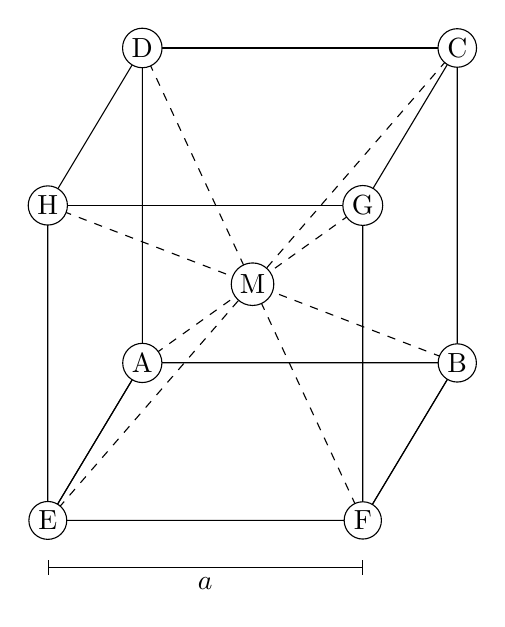
\begin{tikzpicture}[scale=2, z={(-3mm, -5mm)}]
		\coordinate (a) at (0, 0, 0);
		\coordinate (b) at (2, 0, 0);
		\coordinate (c) at (2, 2, 0);
		\coordinate (d) at (0, 2, 0);
		\coordinate (e) at (0, 0, 2);
		\coordinate (f) at (2, 0, 2);
		\coordinate (g) at (2, 2, 2);
		\coordinate (h) at (0, 2, 2);
		\coordinate (m) at (1, 1, 1);

		\draw (a) -- (b) -- (c) -- (d) -- (a);
		\draw (e) -- (f) -- (g) -- (h) -- (e);
		\draw (a) -- (d) -- (h) -- (e) -- (a);
		\draw (b) -- (c) -- (g) -- (f) -- (b);
		\draw (a) -- (b) -- (f) -- (e) -- (a);

		\draw[dashed] (a) -- (m);
		\draw[dashed] (b) -- (m);
		\draw[dashed] (c) -- (m);
		\draw[dashed] (d) -- (m);
		\draw[dashed] (e) -- (m);
		\draw[dashed] (f) -- (m);
		\draw[dashed] (g) -- (m);
		\draw[dashed] (h) -- (m);

		\node[draw, circle, fill=white, inner sep=.5mm] at (a) {A};
		\node[draw, circle, fill=white, inner sep=.5mm] at (b) {B};
		\node[draw, circle, fill=white, inner sep=.5mm] at (c) {C};
		\node[draw, circle, fill=white, inner sep=.5mm] at (d) {D};
		\node[draw, circle, fill=white, inner sep=.5mm] at (e) {E};
		\node[draw, circle, fill=white, inner sep=.5mm] at (f) {F};
		\node[draw, circle, fill=white, inner sep=.5mm] at (g) {G};
		\node[draw, circle, fill=white, inner sep=.5mm] at (h) {H};
		\node[draw, circle, fill=white, inner sep=.5mm] at (m) {M};

		\draw[|-|] (0, -.3, 2) -- ++(2, 0, 0) node[below, midway] {$a$};
	\end{tikzpicture}
	\caption{%
		bcc Zelle. Die Punkte A bis H sind die Eckpunkte, M ist der
		Mittelpunkt.
	}
	\label{fig:bcc}
\end{figure}

\subsection{Basisvektoren des Bravaisgitters}

Es handelt sich hier um einen Würfel mit Kantenlänge $a$, also sind die
Basisvektoren skalierte Versionen der kanonischen Basisvektoren des $\R^3$:
\[
	\vec t_i = a \ev_i
\]

\subsection{Volumina der Zellen}

Die konventionelle Zelle ist die, aus der man den ganzen Kristall durch
Translation aufbauen kann. Dies sollte dann das Parallelepiped sein, das von
den $\vec t_i$ aufgespannt wird. Da diese orthogonal sind und einen Würfel
aufspannen, ist das Volumen $V_\text{konv.} = a^3$.

Die Einheitszelle ist die, bei der nur an den Eckpunkten Atome sitzen. Dies ist
die quadratische Pyramide ABCDM aus Abbildung \ref{fig:bcc}. Das Volumen ist
ein Sechstel des ganzen Würfels, also:
\[
	V_\text{Einh.} = \frac{a^3}6
\]

\subsection{Gitterkonstante bestimmen}

Innerhalb einer konventionellen Zelle sind von den Eckatomen jeweils nur ein
Achtel, allerdings gibt es acht von ihnen. Und das mittlere Atom ist komplett
drin. Also sind pro Einheitszelle gerade zwei volle Atome enthalten. Die
Atomdichte $\nu$ ist also:
\[
	\nu = \frac{2}{a^3}
\]

Mit einer Dichte von $\rho = \SI{10.28}{\gram\per\centi\meter\cubed}$ und einer
Molaren Masse von $\SI{95.9}{\gram\per\mol}$ sind dies
\[
	\nu
	= \SI{107.2}{\milli\mol\per\centi\meter\cubed}
	= \SI{6.455e22}{\per\centi\meter\cubed}
\]

Somit erhalte ich für $a$:
\[
	a = \SI{3.141e-10}{\meter}
\]

Die Gitterkonstante ist also im Bereich einiger Atomradii, was anschaulich gut
passt.

\subsection{Welches Bravaisgitter?}

Das gesamte Gitter, wenn man ignoriert, dass es von zwei verschiedenen Ionen
besetzt ist, ist einfach nur kubisch.

Die Gitter von Chlor und Natrium einzeln sind kubisch flächenzentriert.

\subsection{Vektoren einzeichnen}

Die Vektoren $\vec t_n$ sind in Abbildung \ref{fig:bravaisgitter}, sowie die
Vektoren $\vec d_n$ in Abbildung \ref{fig:einheitszelle}. Dabei bin ich davon
ausgegangen, dass das interessantere Gitter der einzelnen Ionen gemeint ist.
Das kubische Gitter des Gesamtkristalls hat sowohl als Bravaisgitter, als auch
als konventionelle Zelle die gestreckten, kanonischen Basisvektoren des $\R^3$.

\begin{figure}[h]
	\centering
	\begin{tikzpicture}[scale=3, z={(-3mm, -5mm)}]

		\foreach \x in {0, ..., 1}
		\foreach \y in {0, ..., 2}
		\foreach \z in {0, ..., 2}
		\draw (\x, \y, \z) -- ++(1, 0, 0);

		\foreach \x in {0, ..., 2}
		\foreach \y in {0, ..., 1}
		\foreach \z in {0, ..., 2}
		\draw (\x, \y, \z) -- ++(0, 1, 0);

		\foreach \x in {0, ..., 2}
		\foreach \y in {0, ..., 2}
		\foreach \z in {0, ..., 1}
		\draw (\x, \y, \z) -- ++(0, 0, 1);

		\node[fill=white, draw, circle] (n1) at (0, 0, 0) {Na};
		\node[fill=white, draw, circle] (n2) at (2, 0, 0) {Na};
		\node[fill=white, draw, circle] (n3) at (2, 2, 0) {Na};
		\node[fill=white, draw, circle] (n4) at (0, 2, 0) {Na};
		\node[fill=white, draw, circle] (n4) at (1, 1, 0) {Na};
		\node[fill=white, draw, circle] (n1) at (1, 0, 1) {Na};
		\node[fill=white, draw, circle] (n2) at (1, 2, 1) {Na};
		\node[fill=white, draw, circle] (n3) at (2, 1, 1) {Na};
		\node[fill=white, draw, circle] (n4) at (0, 1, 1) {Na};
		\node[fill=white, draw, circle] (n5) at (0, 0, 2) {Na};
		\node[fill=white, draw, circle] (n6) at (2, 0, 2) {Na};
		\node[fill=white, draw, circle] (n7) at (2, 2, 2) {Na};
		\node[fill=white, draw, circle] (n8) at (0, 2, 2) {Na};
		\node[fill=white, draw, circle] (n4) at (1, 1, 2) {Na};

		\draw[->, very thick, color=darkgreen] (0, 0, 2) -- ++(2, 0, 0) node[midway, above, sloped] {$\vec t_1$};
		\draw[->, very thick, color=darkgreen] (0, 0, 2) -- ++(0, 2, 0) node[midway, above, sloped] {$\vec t_3$};
		\draw[->, very thick, color=darkgreen] (0, 0, 2) -- ++(0, 0, -2) node[midway, above, sloped] {$\vec t_2$};

	\end{tikzpicture}
	\caption{%
		Das kubisch flächenzentrierte Gitter des Natriums. Eingezeichnet sind
		die Vektoren, die das Bravaisgitter aufspannen.
	}
	\label{fig:bravaisgitter}
\end{figure}

\begin{figure}[h]
	\centering
	\begin{tikzpicture}[scale=3, z={(-3mm, -5mm)}]

		\foreach \x in {0, ..., 1}
		\foreach \y in {0, ..., 2}
		\foreach \z in {0, ..., 2}
		\draw (\x, \y, \z) -- ++(1, 0, 0);

		\foreach \x in {0, ..., 2}
		\foreach \y in {0, ..., 1}
		\foreach \z in {0, ..., 2}
		\draw (\x, \y, \z) -- ++(0, 1, 0);

		\foreach \x in {0, ..., 2}
		\foreach \y in {0, ..., 2}
		\foreach \z in {0, ..., 1}
		\draw (\x, \y, \z) -- ++(0, 0, 1);

		\node[fill=white, draw, circle] (n1) at (0, 0, 0) {Na};
		\node[fill=white, draw, circle] (n2) at (2, 0, 0) {Na};
		\node[fill=white, draw, circle] (n3) at (2, 2, 0) {Na};
		\node[fill=white, draw, circle] (n4) at (0, 2, 0) {Na};
		\node[fill=white, draw, circle] (n4) at (1, 1, 0) {Na};
		\node[fill=white, draw, circle] (n1) at (1, 0, 1) {Na};
		\node[fill=white, draw, circle] (n2) at (1, 2, 1) {Na};
		\node[fill=white, draw, circle] (n3) at (2, 1, 1) {Na};
		\node[fill=white, draw, circle] (n4) at (0, 1, 1) {Na};
		\node[fill=white, draw, circle] (n5) at (0, 0, 2) {Na};
		\node[fill=white, draw, circle] (n6) at (2, 0, 2) {Na};
		\node[fill=white, draw, circle] (n7) at (2, 2, 2) {Na};
		\node[fill=white, draw, circle] (n8) at (0, 2, 2) {Na};
		\node[fill=white, draw, circle] (n4) at (1, 1, 2) {Na};

		\draw[->, very thick, color=darkblue] (0, 0, 2) -- ++(1, 0, -1) node[midway, above, sloped] {$\vec d_1$};
		\draw[->, very thick, color=darkblue] (0, 0, 2) -- ++(0, 1, -1) node[midway, above, sloped] {$\vec d_3$};
		\draw[->, very thick, color=darkblue] (0, 0, 2) -- ++(0, 0, -2) node[midway, above, sloped] {$\vec d_2$};

	\end{tikzpicture}
	\caption{%
		Das kubisch flächenzentrierte Gitter des Natriums. Eingezeichnet sind
		die Vektoren, die die Einheitszelle aufspannen.
	}
	\label{fig:einheitszelle}
\end{figure}

\subsection{Gitterkonstante von Natriumchlorid}

In einer kubischen Zelle, die die Kantenlänge $a/2$ hat, ist jeweils ein halbes
Chlor- und ein halbes Natriumion enthalten. In einer ganzen konventionellen
Zelle sind also acht mal so viele, also vier Ionenpaare enthalten.

Die Dichte ist $\varrho = \SI{2.17}{\gram\per\centi\meter\cubed}$. Die Masse
pro Ionenpaar ist $m = \SI{9.70e-23}{\gram}$. Das eingenommene Volumen pro
Ionenpaar ist $m/\varrho$, die Größe der Zellen ist $4m/\varrho$. Die
Kubikwurzel daraus ist dann die Gitterkonstante $a = \SI{5.63e-10}\meter$.

%%%%%%%%%%%%%%%%%%%%%%%%%%%%%%%%%%%%%%%%%%%%%%%%%%%%%%%%%%%%%%%%%%%%%%%%%%%%%%%
%                              Reziprokes Gitter                              %
%%%%%%%%%%%%%%%%%%%%%%%%%%%%%%%%%%%%%%%%%%%%%%%%%%%%%%%%%%%%%%%%%%%%%%%%%%%%%%%

\section{Reziprokes Gitter}
\label 3

\subsection{Bravaisvektoren}

Die Bravaisvektoren sind in Abbildung \ref{fig:3a-bravais}. Die Basisvektoren
für die Einheitszelle in Abbildung \ref{fig:3a-basis}. Das Gitter ist in
Abbildung \ref{fig:normal} dargestellt.

\begin{figure}[h]
	\centering
	\begin{tikzpicture}[scale=2]
		\fill[gray] (0, 0) circle (.5mm);
		\fill[gray] (-30:1) circle (.5mm);
		\draw[gray] (-150:1) circle (.5mm);
		\fill[gray] ($(-30:1)+(-90:1)$) circle (.5mm);
		\fill[gray] ($(-30:1)+(30:1)$) circle (.5mm);
		\fill[gray] ($(-30:1)+(-90:1)+(-30:1)+(30:1)$) circle (.5mm);
		\draw[gray] ($(-30:1)+(30:1)+(-30:1)$) circle (.5mm);
		\draw[gray] ($(-30:1)+(-90:1)+(-30:1)$) circle (.5mm);

		\draw[blue, ->, thick] (0, 0) -- (-30:1) node[midway, sloped, above] {$\vec d_1$};
		\draw[blue, ->, thick] (0, 0) -- ($(-30:1)+(-90:1)$) node[midway, sloped, above] {$\vec d_2$};
		\draw[blue, ->, thick] (0, 0) -- ($(-30:1)+(30:1)$) node[midway, sloped, above] {$\vec d_3$};
		\draw[blue, ->, thick] (0, 0) -- ($(-30:1)+(-90:1)+(-30:1)+(30:1)$) node[midway, sloped, above] {$\vec d_4$};

	\end{tikzpicture}
	\caption{%
		Bravaisvektoren für Graphen in blau.
	}
	\label{fig:3a-bravais}
\end{figure}

\begin{figure}[h]
	\centering
	\begin{tikzpicture}[scale=2]
		\fill[gray] (0, 0) circle (.5mm);
		\fill[gray] (-30:1) circle (.5mm);
		\draw[gray] (-150:1) circle (.5mm);
		\fill[gray] ($(-30:1)+(-90:1)$) circle (.5mm);
		\fill[gray] ($(-30:1)+(30:1)$) circle (.5mm);
		\fill[gray] ($(-30:1)+(-90:1)+(-30:1)+(30:1)$) circle (.5mm);
		\draw[gray] ($(-30:1)+(30:1)+(-30:1)$) circle (.5mm);
		\draw[gray] ($(-30:1)+(-90:1)+(-30:1)$) circle (.5mm);

		\draw[red, ->, thick] (0, 0) -- ++(1.732, 0) node[midway, sloped, above] {$\vec t_1$};
		\draw[red, ->, thick] (0, 0) -- ++(.866, -1.5) node[midway, sloped, above] {$\vec t_2$};

	\end{tikzpicture}
	\caption{%
		Basisvektoren für die Einheitszelle in rot.
	}
	\label{fig:3a-basis}
\end{figure}

\begin{figure}[h]
	\centering
	\begin{tikzpicture}[scale=.25]
		\foreach \x in {0, ..., 3}
		\foreach \y in {0, ..., 3}
		\draw ($\x*(10.88, 0)+\y*(5.44, -9.43)$) circle (4mm);
	\end{tikzpicture}
	\caption{%
		Das normale Gitter
	}
	\label{fig:normal}
\end{figure}

In kartesischen Koordinaten sind die Bravaisvektoren:
\[
	\vec t_1 =
	\begin{pmatrix}
		\sqrt 3 \\ 0
	\end{pmatrix}
	a
	\eqnsep
	\vec t_2 =
	\begin{pmatrix}
		\sqrt 3/2 \\ -3/2
	\end{pmatrix}
	a
\]

Und die Basisvektoren:
\[
	\vec d_1 =
	\begin{pmatrix}
		\sqrt 3/2 \\ - 1/2
	\end{pmatrix}
	a
	\eqnsep
	\vec d_2 = \vec t_2
	\eqnsep
	\vec d_3 = \vec t_1
	\eqnsep
	\vec d_4 =
	\begin{pmatrix}
		3\sqrt3/2 \\ -1/5
	\end{pmatrix}
	a
\]

\subsection{Reziprokes Gitter}

Das reziproke Gitter $\vec g_i$ hat als definierende Eigenschaft:
\[
	\inner{\vec t_i}{\vec g_j} = 2 \piup \delta_{ij}
\]

Laut \cite{wikipedia/Reziprokes_Gitter} kann ich die Bravaisvektoren in eine
Matrix $2 \piup \tens A$ schreiben, transponieren, invertieren und erhalte eine
Matrix $\tens B$, in der die Vektoren des reziproken Gitters stehen:
\[
	\tens B = \del{2 \piup \tens A^\text T}^{-1}
\]

Die Vektoren $\vec g_i$ aus dem reziproken Gitter sind:
\[
	\vec g_1 = \frac{2 \piup}a
	\begin{pmatrix}
		\frac{1}{\sqrt3} \\ \frac 13
	\end{pmatrix}
	\eqnsep
	\vec g_2 = \frac{2 \piup}a
	\begin{pmatrix}
		0 \\ - \frac 23
	\end{pmatrix}
\]

Das reziproke Gitter ist in Abbildung \ref{fig:3b} dargestellt.

\begin{figure}[h]
	\centering
	\begin{tikzpicture}[scale=.5]
		\foreach \x in {0, ..., 4}
		\foreach \y in {0, ..., 4}
		\draw ($\x*(3.63, 2.09)+\y*(0, -4.19)$) circle (2mm);
	\end{tikzpicture}
	\caption{%
		Gitterpunkte des reziproken Gitters.
	}
	\label{fig:3b}
\end{figure}

\subsection{Erste Brillouinzone}

Laut \cite{wikipedia/Brillouin-Zone} kann ich die Brillouinzone konstruieren,
in dem ich mir einen Punkt aus dem Gitter aussuche und zu jedem Nachbarpunkt
die Mittelsenkrechte einzeichne. Die Fläche, die sich dann ergibt, ist die
erste Brilloinzone. Die Nachbarn sind in Abbildung \ref{fig:3c-1} dargestellt.
Die Zone ist in Abbildung \ref{fig:3c-2} konstruiert.

\begin{figure}[h]
	\centering
	\begin{tikzpicture}[scale=.5]
		\coordinate (m) at ($1*(3.63, 2.09)+1*(0, -4.19)$);
		\coordinate (1) at ($0*(3.63, 2.09)+0*(0, -4.19)$);
		\coordinate (2) at ($1*(3.63, 2.09)+0*(0, -4.19)$);
		\coordinate (3) at ($2*(3.63, 2.09)+1*(0, -4.19)$);
		\coordinate (4) at ($2*(3.63, 2.09)+2*(0, -4.19)$);
		\coordinate (5) at ($1*(3.63, 2.09)+2*(0, -4.19)$);
		\coordinate (6) at ($0*(3.63, 2.09)+1*(0, -4.19)$);

		\node[draw, circle] at (m) {m};
		\node[draw, circle] at (1) {1};
		\node[draw, circle] at (2) {2};
		\node[draw, circle] at (3) {3};
		\node[draw, circle] at (4) {4};
		\node[draw, circle] at (5) {5};
		\node[draw, circle] at (6) {6};
	\end{tikzpicture}
	\caption{%
		Unmittelbare Nachbarn eines Punktes im reziproken Gitter.
	}
	\label{fig:3c-1}
\end{figure}

\begin{figure}[h]
	\centering
	\begin{tikzpicture}[scale=.5]
		\coordinate (m) at ($1*(3.63, 2.09)+1*(0, -4.19)$);
		\coordinate (1) at ($0*(3.63, 2.09)+0*(0, -4.19)$);
		\coordinate (2) at ($1*(3.63, 2.09)+0*(0, -4.19)$);
		\coordinate (3) at ($2*(3.63, 2.09)+1*(0, -4.19)$);
		\coordinate (4) at ($2*(3.63, 2.09)+2*(0, -4.19)$);
		\coordinate (5) at ($1*(3.63, 2.09)+2*(0, -4.19)$);
		\coordinate (6) at ($0*(3.63, 2.09)+1*(0, -4.19)$);

		\node[fill, circle] at (m) {};
		\node[fill, circle] at (1) {};
		\node[fill, circle] at (2) {};
		\node[fill, circle] at (3) {};
		\node[fill, circle] at (4) {};
		\node[fill, circle] at (5) {};
		\node[fill, circle] at (6) {};

		\draw (1) -- (3);
		\draw (2) -- (4);
		\draw (3) -- (5);
		\draw (4) -- (6);
		\draw (5) -- (1);
		\draw (6) -- (2);
	\end{tikzpicture}
	\caption{%
		Konstruktion der ersten Brilloinzone. Die Fläche um den zentralen Punkt
		ist die gesuchte Zone.
	}
	\label{fig:3c-2}
\end{figure}

\subsection{Millerindizes}

Wenn ich \cite{wikipedia/Millersche_Indizes} richtig verstanden habe, dann sind
die Millerindizes letztlich die inversen Spurpunkte der Ebene.

Die Hyperebene zu $(10)$ sollte dann also bei $\vec t_1$ den Spurpunkt 1 und
bei $\vec t_2$ den Spurpunkt $\infty$ haben, also parallel dazu sein. Sie sind
in Abbildungen \ref{fig:10}, \ref{fig:11}, \ref{fig:21} sowie \ref{fig:01}
eingezeichnet.

\begin{figure}[h]
	\centering
	\begin{tikzpicture}[scale=.25]
		\foreach \x in {0, ..., 1}
		\foreach \y in {0, ..., 1}
		\draw ($\x*(10.88, 0)+\y*(5.44, -9.43)$) circle (4mm);
		\draw[thick, red] ($1*(10.88, 0)+0*(5.44, -9.43)$) -- ($1*(10.88, 0)+1*(5.44, -9.43)$);
	\end{tikzpicture}
	\caption{%
		Hyperebene zum Millerindex $(10)$.
	}
	\label{fig:10}
\end{figure}

\begin{figure}[h]
	\centering
	\begin{tikzpicture}[scale=.25]
		\foreach \x in {0, ..., 1}
		\foreach \y in {0, ..., 1}
		\draw ($\x*(10.88, 0)+\y*(5.44, -9.43)$) circle (4mm);
		\draw[thick, red] ($0*(10.88, 0)+1*(5.44, -9.43)$) -- ($1*(10.88, 0)+0*(5.44, -9.43)$);
	\end{tikzpicture}
	\caption{%
		Hyperebene zum Millerindex $(11)$.
	}
	\label{fig:11}
\end{figure}

\begin{figure}[h]
	\centering
	\begin{tikzpicture}[scale=.25]
		\foreach \x in {0, ..., 1}
		\foreach \y in {0, ..., 1}
		\draw ($\x*(10.88, 0)+\y*(5.44, -9.43)$) circle (4mm);
		\draw[thick, red] ($0*(10.88, 0)+1*(5.44, -9.43)$) -- ($.5*(10.88, 0)+0*(5.44, -9.43)$);
	\end{tikzpicture}
	\caption{%
		Hyperebene zum Millerindex $(21)$.
	}
	\label{fig:21}
\end{figure}

\begin{figure}[h]
	\centering
	\begin{tikzpicture}[scale=.25]
		\foreach \x in {0, ..., 1}
		\foreach \y in {0, ..., 1}
		\draw ($\x*(10.88, 0)+\y*(5.44, -9.43)$) circle (4mm);
		\draw[thick, red] ($0*(10.88, 0)+1*(5.44, -9.43)$) -- ($1*(10.88, 0)+1*(5.44, -9.43)$);
	\end{tikzpicture}
	\caption{%
		Hyperebene zum Millerindex $(01)$.
	}
	\label{fig:01}
\end{figure}

%%%%%%%%%%%%%%%%%%%%%%%%%%%%%%%%%%%%%%%%%%%%%%%%%%%%%%%%%%%%%%%%%%%%%%%%%%%%%%%
%                     Bragg-Beugung und Röntgenstrahlung                     %
%%%%%%%%%%%%%%%%%%%%%%%%%%%%%%%%%%%%%%%%%%%%%%%%%%%%%%%%%%%%%%%%%%%%%%%%%%%%%%%

\section{Bragg-Beugung und Röntgenstrahlung}
\label 4

\subsection{Reziprokes Gitter}

Da hier die Gittervektoren einfach die kanonischen Einheitsvektoren sind, unterscheiden sich die Vektoren des reziproken Gitters nur durch einen Faktor. Die Vektoren sind also:
\[
	\vec g_1 = \frac{2\piup}a \ev_x
	\eqnsep
	\vec g_2 = \frac{2\piup}a \ev_y
	\eqnsep
	\vec g_3 = \frac{2\piup}a \ev_z
\]

\subsection{Hyperebenenfamilie}

Die Ebene $(110)$ hat die Spurpunkte $(1, 1, \infty)$. Es sind also die
$x$-$y$-Ebenen. Sie sind in Abbildung \ref{fig:millerebenen} eingezeichnet.

\begin{figure}[h]
	\centering
	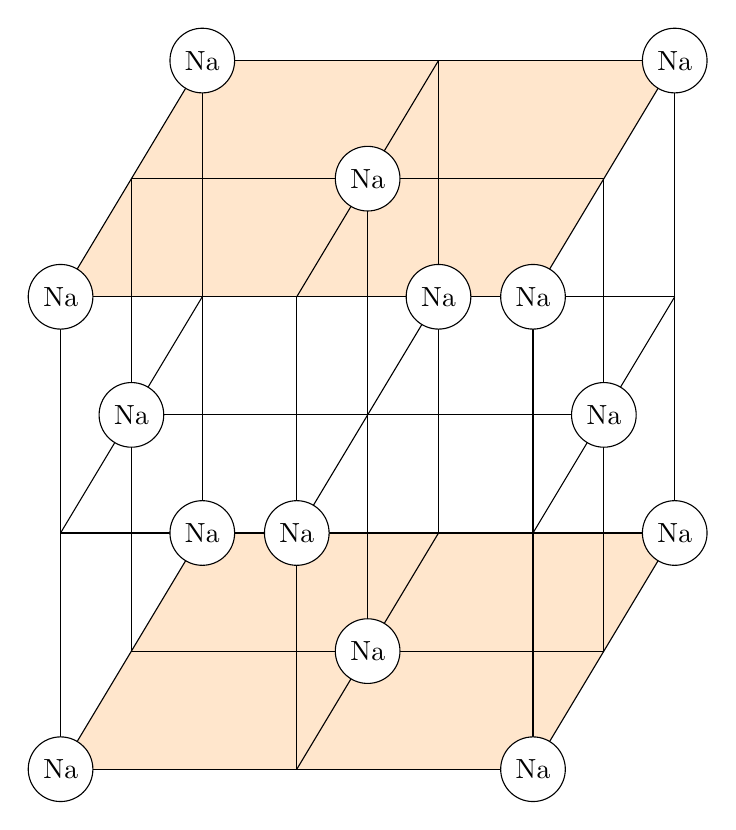
\begin{tikzpicture}[scale=3, z={(-3mm, -5mm)}]
		\fill[opacity=.2, color=orange] (0, 0, 0) -- (2, 0, 0) -- (2, 0, 2) -- (0, 0, 2) -- cycle;
		\fill[opacity=.2, color=orange] (0, 2, 0) -- (2, 2, 0) -- (2, 2, 2) -- (0, 2, 2) -- cycle;

		\foreach \x in {0, ..., 1}
		\foreach \y in {0, ..., 2}
		\foreach \z in {0, ..., 2}
		\draw (\x, \y, \z) -- ++(1, 0, 0);

		\foreach \x in {0, ..., 2}
		\foreach \y in {0, ..., 1}
		\foreach \z in {0, ..., 2}
		\draw (\x, \y, \z) -- ++(0, 1, 0);

		\foreach \x in {0, ..., 2}
		\foreach \y in {0, ..., 2}
		\foreach \z in {0, ..., 1}
		\draw (\x, \y, \z) -- ++(0, 0, 1);

		\node[fill=white, draw, circle] (n1) at (0, 0, 0) {Na};
		\node[fill=white, draw, circle] (n2) at (2, 0, 0) {Na};
		\node[fill=white, draw, circle] (n3) at (2, 2, 0) {Na};
		\node[fill=white, draw, circle] (n4) at (0, 2, 0) {Na};
		\node[fill=white, draw, circle] (n4) at (1, 1, 0) {Na};
		\node[fill=white, draw, circle] (n1) at (1, 0, 1) {Na};
		\node[fill=white, draw, circle] (n2) at (1, 2, 1) {Na};
		\node[fill=white, draw, circle] (n3) at (2, 1, 1) {Na};
		\node[fill=white, draw, circle] (n4) at (0, 1, 1) {Na};
		\node[fill=white, draw, circle] (n5) at (0, 0, 2) {Na};
		\node[fill=white, draw, circle] (n6) at (2, 0, 2) {Na};
		\node[fill=white, draw, circle] (n7) at (2, 2, 2) {Na};
		\node[fill=white, draw, circle] (n8) at (0, 2, 2) {Na};
		\node[fill=white, draw, circle] (n4) at (1, 1, 2) {Na};

	\end{tikzpicture}
	\caption{%
		Die Hyperebenenfamilie $(110)$.
	}
	\label{fig:millerebenen}
\end{figure}

\subsection{Abstand der Gitterebenen}

Der Abstand der Gitterebenen ist aus der Zeichnung auf dem Aufgabenblatt zu
entnehmen, er ist das Ergebnis aus der vorherigen Aufgabe, $a =
\SI{5.63e-10}\meter$.

\subsection{Energie der $K_\alpha$ Strahlung}

Bei der $K_\alpha$ Linie wird ein Elektron aus dem $n=1$ Orbital geworfen, und
ein anderes rückt aus $n=2$ nach. Mit der größeren, so nah am Kern nicht
abgeschrimten Kernladung von $Z$ ergibt sich als Energiedifferenz:
\[
	E_{K_\alpha} = Z E_\text{Ryd} \del{\frac1{1^2} - \frac1{2^2}}
	= \SI{428.4}\electronvolt
\]

\subsection{Streuwinkel}

Nach \cite[Seite 862]{meschede-gerthsen_24} gilt für einen beliebigen Vektor aus dem reziproken Gitter:
\[
	\Deltaup \vec k = \vec g
\]

Der einfallende Strahl liege in $x$-$z$-Ebene, der Kristall parallel zur
$x$-$y$-Ebene. Er trifft von oben auf den Kristall im Winkel $\theta$ und
verlässt den Kristall ebenfalls im Winkel $\theta$. Als Änderungen kommt nur
die $z$-Komponente in Frage, so dass der Vektor aus dem reziproken Gitter ein
Vielfaches von $\vec g_3$ sein muss:
\begin{align*}
	\Deltaup \vec k &= \frac{2\piup}a n \ev_z \\
	k \begin{pmatrix}
		\cos\theta \\ 0 \\ \sin\theta
	\end{pmatrix} - k \begin{pmatrix}
		\cos\theta \\ 0 \\ - \sin\theta
	\end{pmatrix} &= \frac{2\piup}a n \ev_z \\
		2k \sin\theta &= \frac{2\piup}a n \\
		\sin\del\theta &= \frac{n\piup}{ak} \\
		\intertext{%
			Mit $k = 2\piup/\lambda$ erhalte ich:
		}
		\sin\del\theta &= \frac{n\lambda}{2a}
\end{align*}

Dies ist die Bragg-Bedingung. Damit stelle ich jetzt eine Tabelle für $\theta$
in $\si\degree$ auf:
\begin{center}
	\begin{tabular}{S|SS}
		{$n$} & {$\lambda_\alpha = \SI{.711}\angstrom$} & {$\lambda_\alpha = \SI{.631}\angstrom$} \\
		\hline
		1 & 3.62029 & 3.21249 \\
		2 & 7.25513 & 6.43513 \\
		3 & 10.9196 & 9.67837 \\
		4 & 14.63 & 12.9533 \\
	\end{tabular}
\end{center}

Die drei gegebenen Streuwinkel liegen dort gut drin. Wenn ich mit diesen $n$ und $\lambda$ sowie den Winkeln $\theta$ die Gitterkonstante $a$ ausrechne, erhalte ich:
\[
	a = \SI{5.64321}\angstrom
	\eqnsep
	a = \SI{5.6417}\angstrom
	\eqnsep
	a = \SI{5.63996}\angstrom
\]

%%%%%%%%%%%%%%%%%%%%%%%%%%%%%%%%%%%%%%%%%%%%%%%%%%%%%%%%%%%%%%%%%%%%%%%%%%%%%%%
%                                    Ende                                     %
%%%%%%%%%%%%%%%%%%%%%%%%%%%%%%%%%%%%%%%%%%%%%%%%%%%%%%%%%%%%%%%%%%%%%%%%%%%%%%%

\IfFileExists{\bibliographyfile}{
	\bibliography{\bibliographyfile}
}{}

\end{document}

% vim: spell spelllang=de
